
% \documentclass[11pt]{article}
% 
% \setlength{\oddsidemargin}{0in}
% \setlength{\evensidemargin}{0in}
% \setlength{\topmargin}{0.0in}
% \setlength{\textwidth}{6.5in}
% \setlength{\textheight}{9.0in}
% \setlength{\parindent}{0in}
% \setlength{\parskip}{0.15in}
% 
% \usepackage{times}
% \usepackage{url}
% 
% \usepackage{listings}
% 
% \usepackage{graphicx}
% 
% \begin{document}
% 
% \title{Introduction to ggplot2}
% 
% \author{N. Matloff}
 
% \date{January 11, 2013}
% 
% \maketitle

\chapter{Introduction to the ggplot2 Graphics Package}
\label{ggplot2}

\section{Introduction}

Hadley Wickham's {\bf ggplot2} package is a hugely popular alternative to
R's base graphics package.  (Others include {\bf lattice}, {\bf ggobi}
and so on.)  

The {\bf ggplot2} pacakge is an implementation of the ideas in the book,
{\it The Grammar of Graphics}, by Leland Wilkison, whose goal was to set
out a set of general unifying principles for the visualization of data.
For this reason, {\bf ggplot2} offers a more elegant and arguably more
natural approach than does the base R graphics package.

The package has a relatively small number of primitive functions, making
it relatively easy to master.  But through combining these functions in
various ways, a very large number of types of graphs may be produced.
It is considered especially good in setting reasonable default values of
parameters, and much is done without the user's asking.  Legends are
automatically added to graphs, for instance.

The package is quite extensive (only a few functions, but lots of
options), and thus this document is merely a brief introduction.

\section{Installation and Use}

Download and install {\bf ggplot2} with the usual {\bf
install.packages()} function, and then at each usage, load via {\bf
library()}.  Here's what I did on my netbook:

\begin{lstlisting}
# did once:
> install.packages("ggplot2","/home/nm/R")
# do each time I use the package (or set in .Rprofile)
> .libPaths("/home/nm/R")
> library(ggplot2)
\end{lstlisting}

\section{Basic Structures}

One operates in the following pattern:

\begin{itemize}

\item One begins with a call to {\bf ggplot()}: 

\begin{lstlisting}
> p <- ggplot(yourdataframe)
\end{lstlisting}

or 

\begin{lstlisting}
> p <- ggplot(yourdataframe,aes(yourargs))
\end{lstlisting}

Here {\bf yourdataframe} could have been read from a file, say using
{\bf read.table()}, or generated within the program.  If your data is in
the form of an R matrix, use {\bf as.data.frame()} to convert it.

The result {\bf p} is an R S3 object of class {\bf "ggplot"}, consisting
of a component named {\bf data}, and other components containing
information about the plot.  

Note that at this point, though, there is nothing to plot (if we didn't
call {\bf aes()}).

\item One adds features to---or even changes---the plot via the {\bf +}
operator, which of course is an overloaded version of R's built-in {\bf
+}, the function {\bf "+.ggplot"()}.  

Each invocation of {\bf +} adds a new {\it layer} to the graph, adding
to the contents of the previous layer.  Typically, each new layer adds
new features to the graph, or changes old features.  One might, for
instance, superimpose several curves on the same graph, by adding one
new layer per curve.\footnote{There are ways to do this in a single
layer, but let's not get too complex in this introductory document.}

The idea of layering is partly motivated by reusability.  One can save a
lower layer in a variable (or on disk, using the R {\bf save()}
function), so that we can make a different graph, with different
features, starting with the same layer.

To actually display a plot, we print it, i.e. print {\bf p}.  Recall
that in R, {\bf print()} is a {\it generic} function, i.e. a stub for a
class-specific one.  In this case the latter does a plot.  At this
stage, we don't have anything to display yet, if we didn't call {\bf
aes()} above.

\item The function {\bf aes()} (``aesthetics'') is used to specify
graph attributes.  For instance, in a scatter plot, which variable will
be on the horizontal axis, and which on the vertical?  What colors do we
want for the points?  Etc.

We can call {\bf aes()} at various layers, depending on how general
(reusable, as noted above) we want each layer to be.  

So for instance we could use {\bf aes()} to specify our data variables
either when we call {\bf ggplot()}, so these variables will be used in
all operations, or when we later add a layer calling, say, {\bf
geom\_point()}, to indicate data variables for this specific operation.

\end{itemize}

There are various types of objects that can be used as the second
operand for the + operator.  Examples are:

\begin{itemize}

\item {\bf geoms} (``geometrics''):  Geometric objects to be drawn, such
as points, lines, bars, polygons and text.

\item {\bf position adjustments}:  For instance, in a bar graph, this
controls whether bars should be side by side, or stacked on top of each
other.

\item {\bf facets}:  Specifications to draw many graphs together, as
panels in a large graph.  You can have rows of panels, columns of
panels, and rows and columns of panels.

\item {\bf themes}:  Don't like the gray background in a graph?  Want
nicer labeling, etc.?  You can set each of these individually, but one
of the built-in themes, or a user-contributed one, can save you the
trouble, or you can write one that you anticipate using a lot.

\end{itemize}

\section{Example:  Simple Line Graphs}

\begin{lstlisting}
> df1
  u v
1 0 3
2 2 4
3 5 5
> ggplot(df1) + geom_line(aes(x=u,y=v))
\end{lstlisting}

Here {\bf aes()} was called from {\bf geom\_line()} rather than from
{\bf ggplot()}, so as to apply just to this line.  The result is

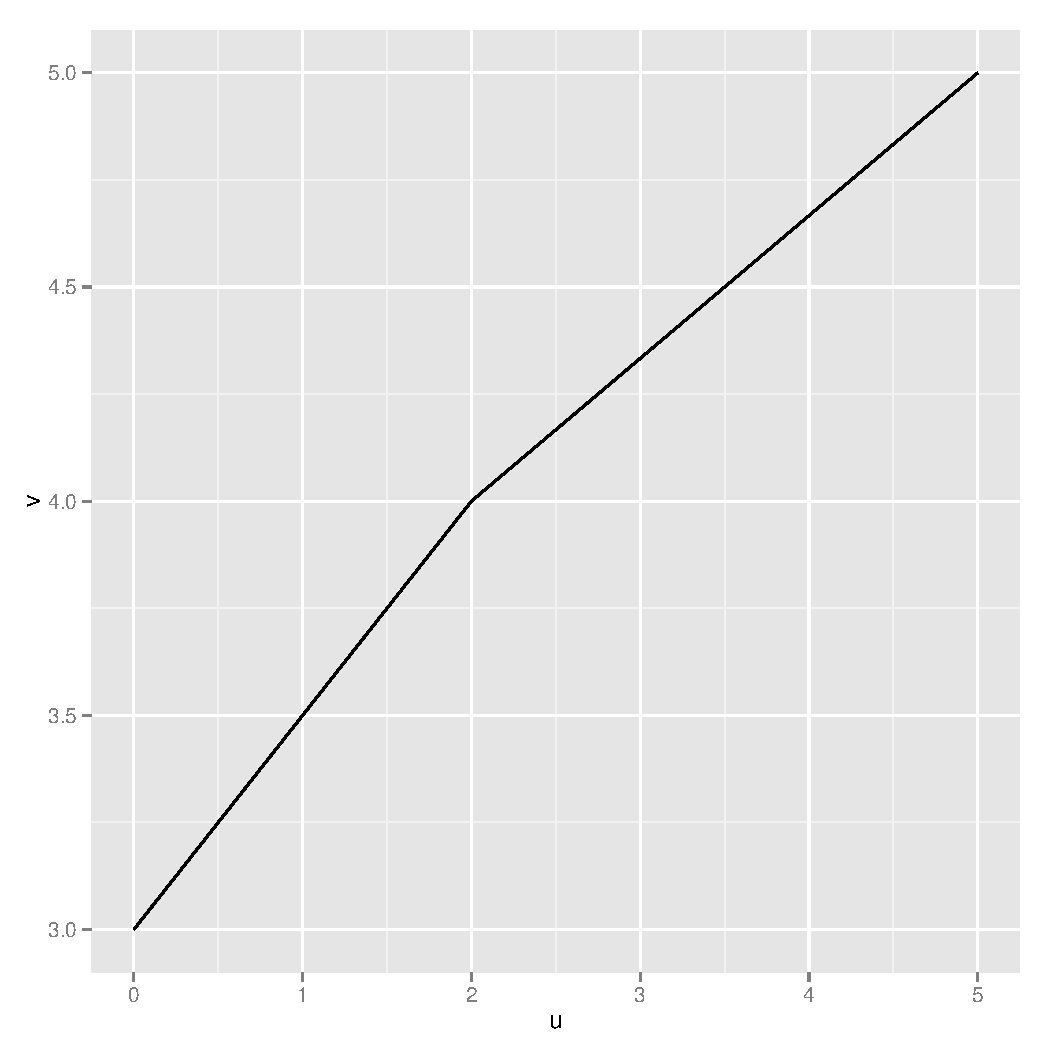
\includegraphics[width=4.0in]{Lines1.pdf}

Now let's add a second line, from a {\it different} data frame:

\begin{lstlisting}
> df2
  w z
1 1 4
2 2 5
3 3 9
ggplot(df1) + geom_line(aes(x=u,y=v)) + geom_line(data=df2,aes(x=w,y=z))
\end{lstlisting}

Here is the result:

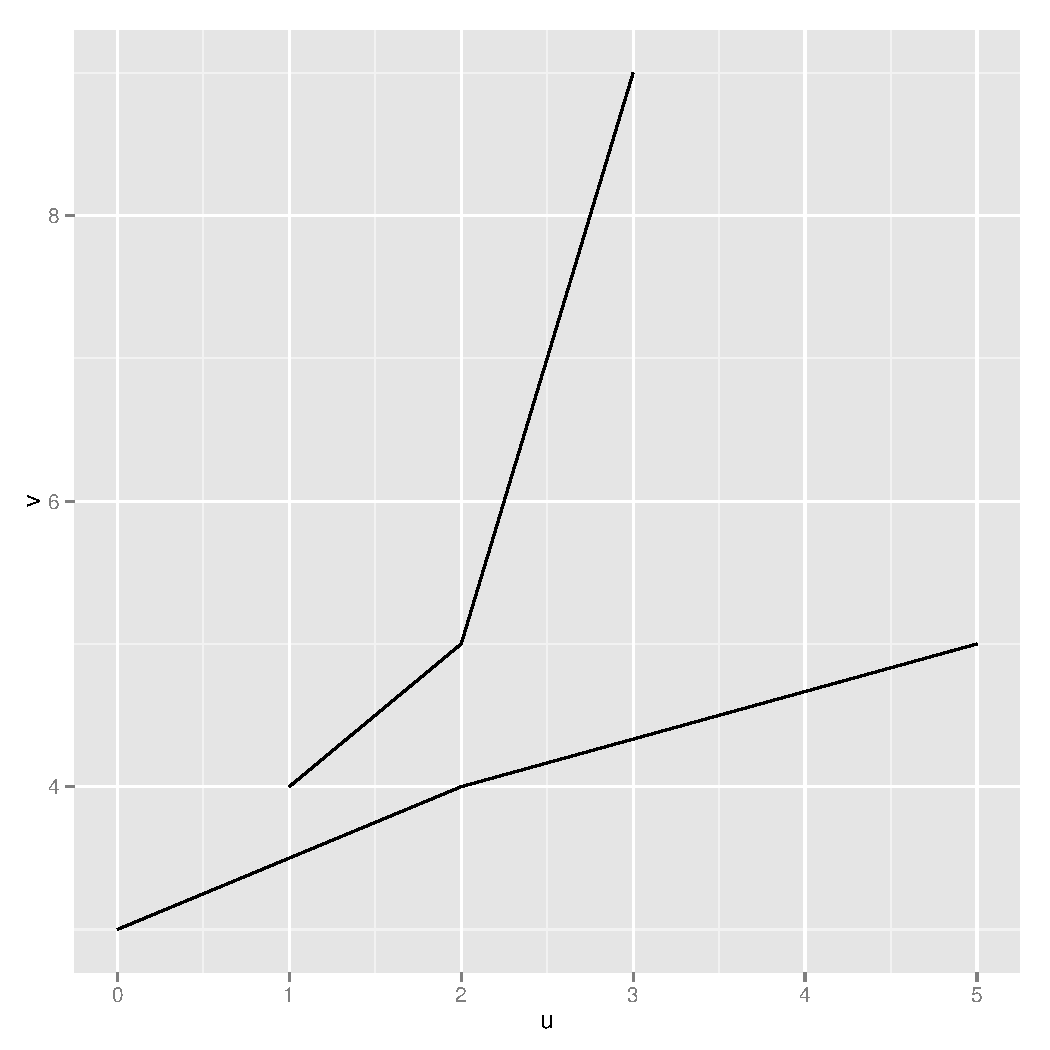
\includegraphics[width=4.0in]{Lines2.pdf}

It worked as long as we specified {\bf data} for the second line.

Note that {\bf ggplot2} automatically adjusted that second graph, to
make room for the ``taller'' second line.

\section{Example:  Census Data}

The data set here consists of programmers (software engineers, etc.) and
electrical engineers in Silicon Valley, in the 2000 Census.  I've
removed those with less than a Bachelor's degree.  The R object was a
data frame named {\bf pm}.

I first ran

\begin{lstlisting}
p <- ggplot(pm)
\end{lstlisting}

to set up the {\bf ggplot} object.  Next, I typed

\begin{lstlisting}
p + geom_histogram(aes(HiDeg))
\end{lstlisting}

which produced a histogram of a particular variable in the data (i.e. a
particular column in the data frame), which was the highest-degree
values of the workers:

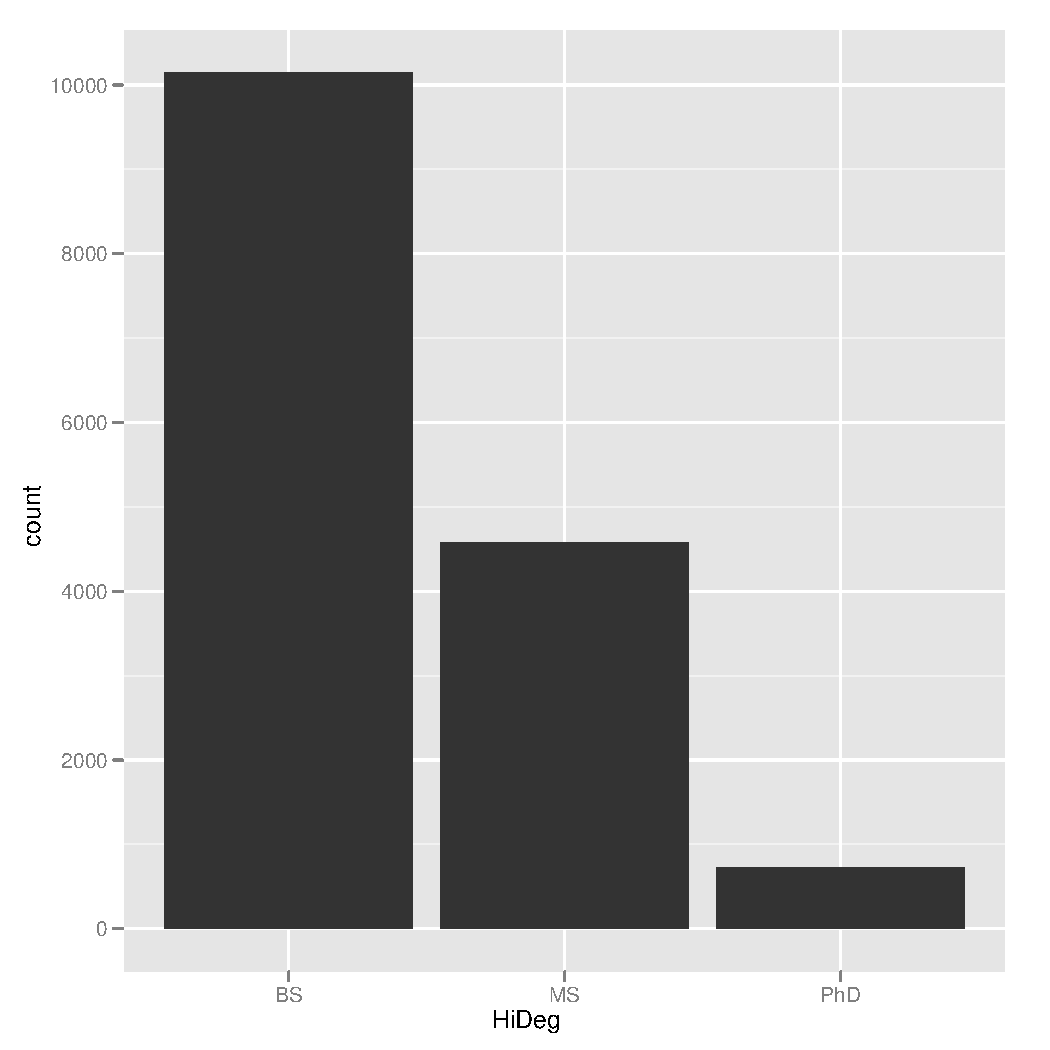
\includegraphics[bb=0 0 504 504,width=4.0in]{EdHist.pdf}

Note that the + operation yields a new object of class {\bf "ggplot"}.
Since the generic print function for that class actually plots the
graph, the graph did appear on the screen.  I could have saved the new
object in a variable if needed.

I then decided to do a scatter plot of salary versus age:

\begin{lstlisting}
> p + geom_point(aes(x=Age,y=WgInc))
\end{lstlisting}

So, here is an example of the reusability mentioned earlier.  For this
small data set, it wasn't an issue, but some larger data sets can take a
while to render, so you definitely want to save intermediate results for
reuse.

Note the roles of {\bf aes()} both here and in the previous example.  I
used it to specify for the geom what I wanted to do in that layer.  Each
geom has its own set of aesthetics one can specify.  In the case of {\bf
geom\_point()}, I need to specify which variable to use for the X- and
Y-axes.  There are other aesthetics for this geom that could be
specified, as you'll see below.

This gave me this graph:

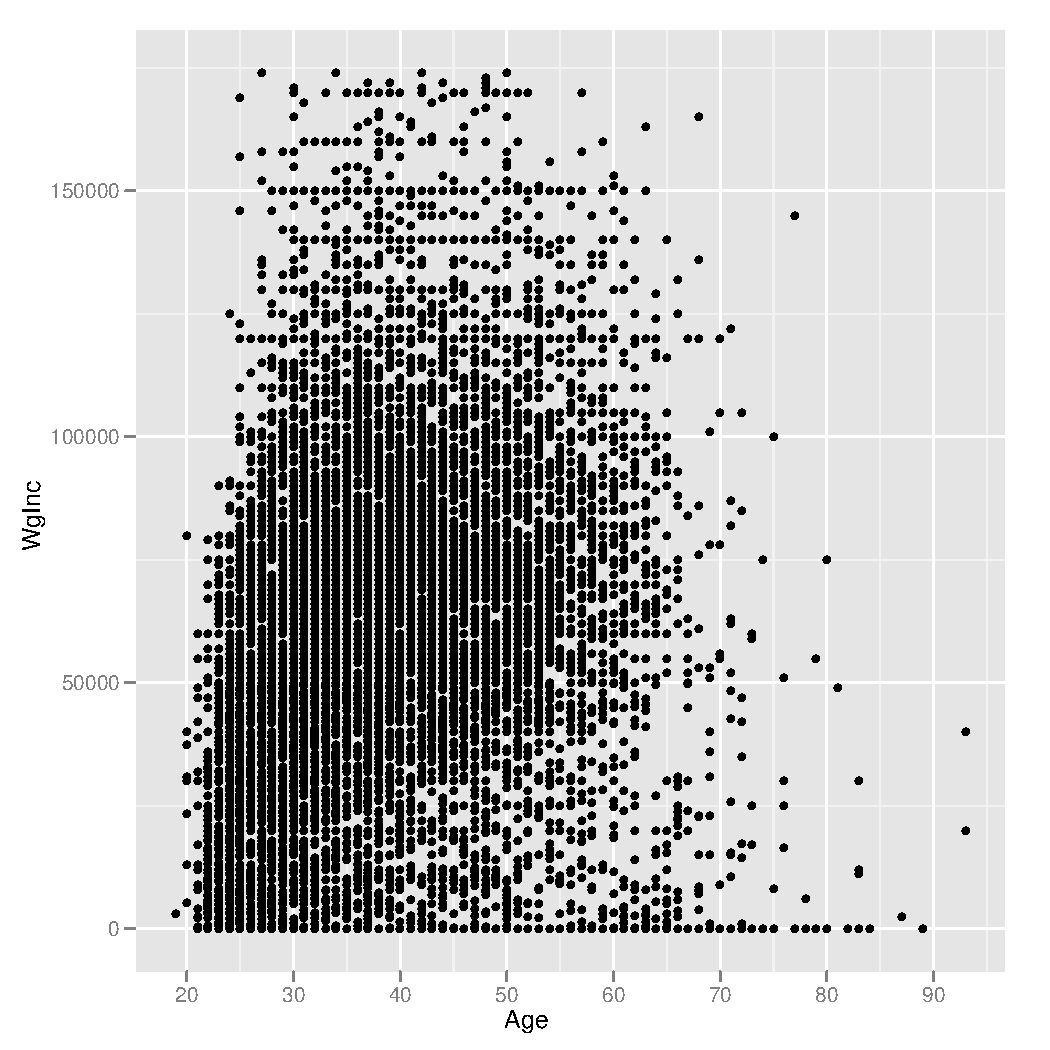
\includegraphics[bb=0 0 504 504,width=3.5in]{AgeInc.pdf}

(As is often the case with large data sets, the points tend to ``fill
in'' entire regions.  One solution is to graph a random subset of the
data, not done here.  Data smoothing techniques can also be used.
Similar comments apply to some of the graphs below.)

However, I wanted to separate the points according to highest degree
level:

\begin{lstlisting}
> p + geom_point(aes(x=Age,y=WgInc,color=HiDeg))
\end{lstlisting}

Here I have three data variables informing {\bf aes()}:  Age, wage
income and highest degree.  The argument {\bf color} here means that I
want the degree to be used for color coding the points:

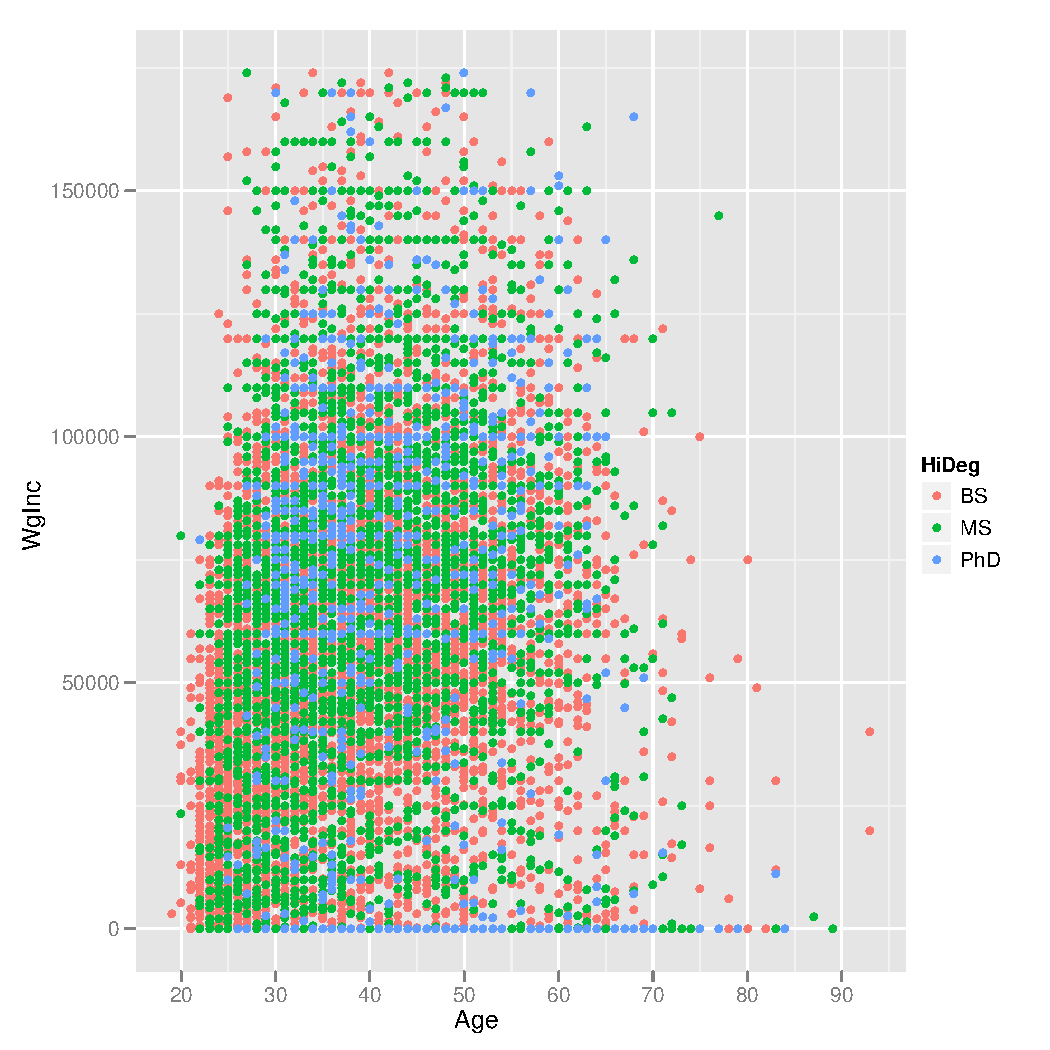
\includegraphics[bb=0 0 504 504,width=3.5in]{AgeIncColor.pdf}

So the orange points are for Bachelor's people, green for Master's and
blue for PhDs.  Note the color legend that was automatically included
on the right.

Since some people might be viewing a black-and-white version of this
document, I ran the command again, specifying coding the highest degree
by point shape instead of point color:

\begin{lstlisting}
p + geom_point(aes(x=Age,y=WgInc,shape=HiDeg))
\end{lstlisting}

Here {\bf ggplot2} decided to use a circle, a triangle and a square to
represent Bachelor's, Master's and PhD workers:

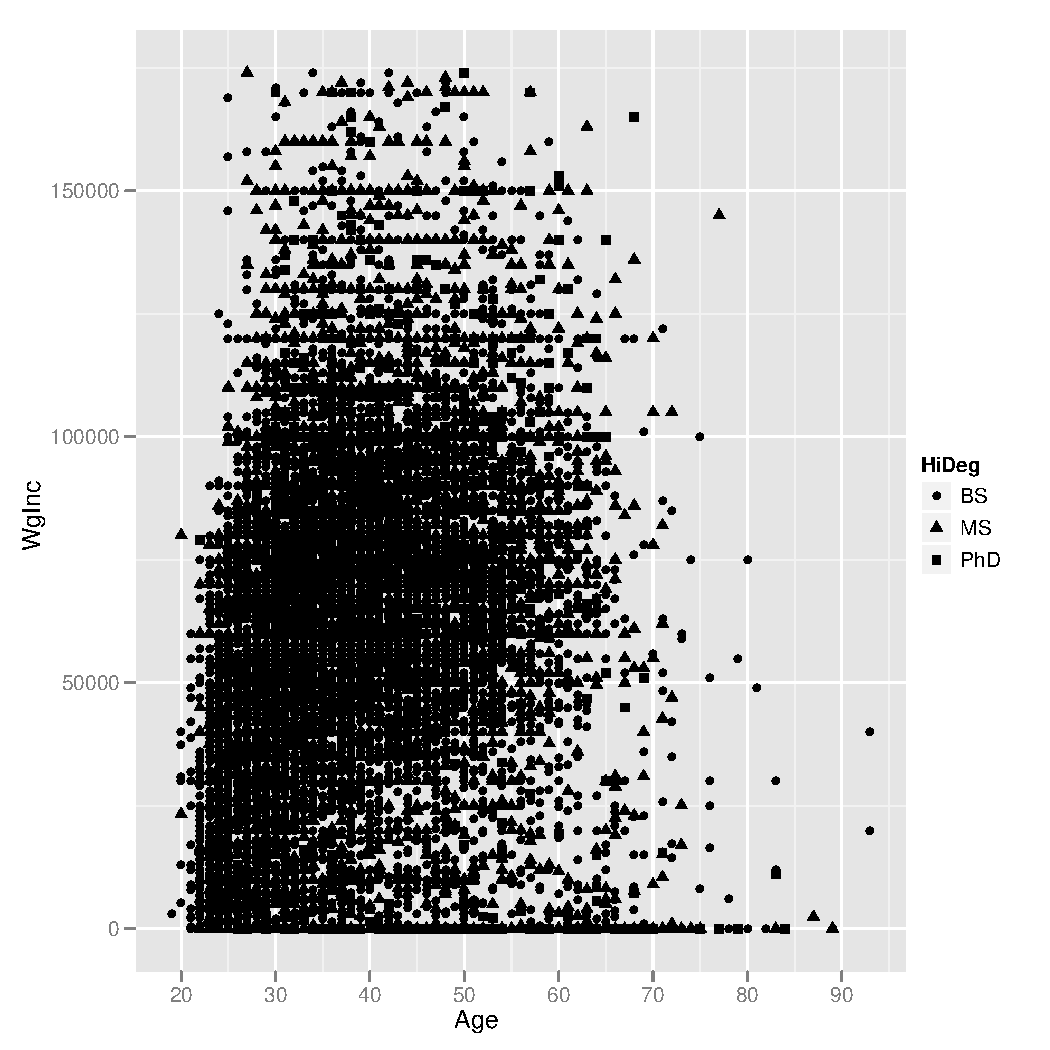
\includegraphics[bb=0 0 504 504,width=4.5in]{AgeIncShape.pdf}

Since I'm interested in age discrimination in the industry, I decided to
restrict my graph to those over age 40.  The {\bf ggplot2} package
cleverly exploits the R {\bf subset()} function, allowing me to write

\begin{lstlisting}
p %+% subset(pm,Age > 40) + geom_point(aes(x=Age,y=WgInc,color=HiDeg))
\end{lstlisting}

The new operator {\bf \%+\%} is again mapped to {\bf "+.ggplot"()}.  The
result was

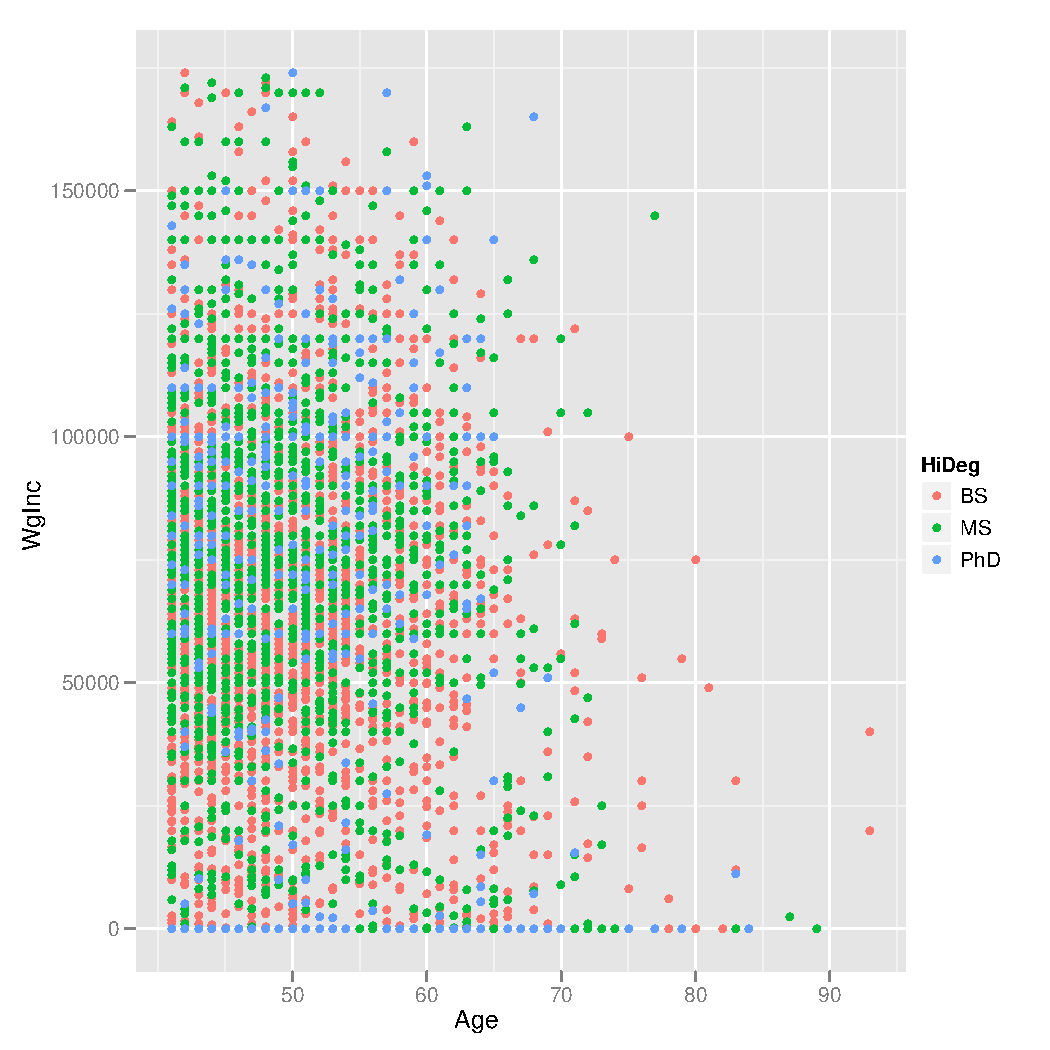
\includegraphics[bb=0 0 504 504,width=4.5in]{40AgeIncColor.pdf}

Look at all those 0-income PhDs!  (There was also a business income
variable, which I did not pursue here, so maybe some had high incomes
after all.)

Even with color, it's a little hard to compare the three degree levels,
so let's try faceting:

\begin{lstlisting}
> pt <- p + geom_point(aes(x=Age, y=WgInc))
> pt + facet_grid(HiDeg ~ .)
\end{lstlisting}

Here I saved an overall graph of wage income versus age to {\bf pt}, and
then added faceting by degree.  This instructed {\bf ggplot2} to draw
three graphs, one for each degree level, as three panels in the same
large graph.  The \lstinline{HiDeg ~ .} argument (which you may
recognize as similar notation to R's {\bf lm()} function for linear
models) states that I want HiDeg to define the rows of panels, without
any variable defining columns.  The result was:

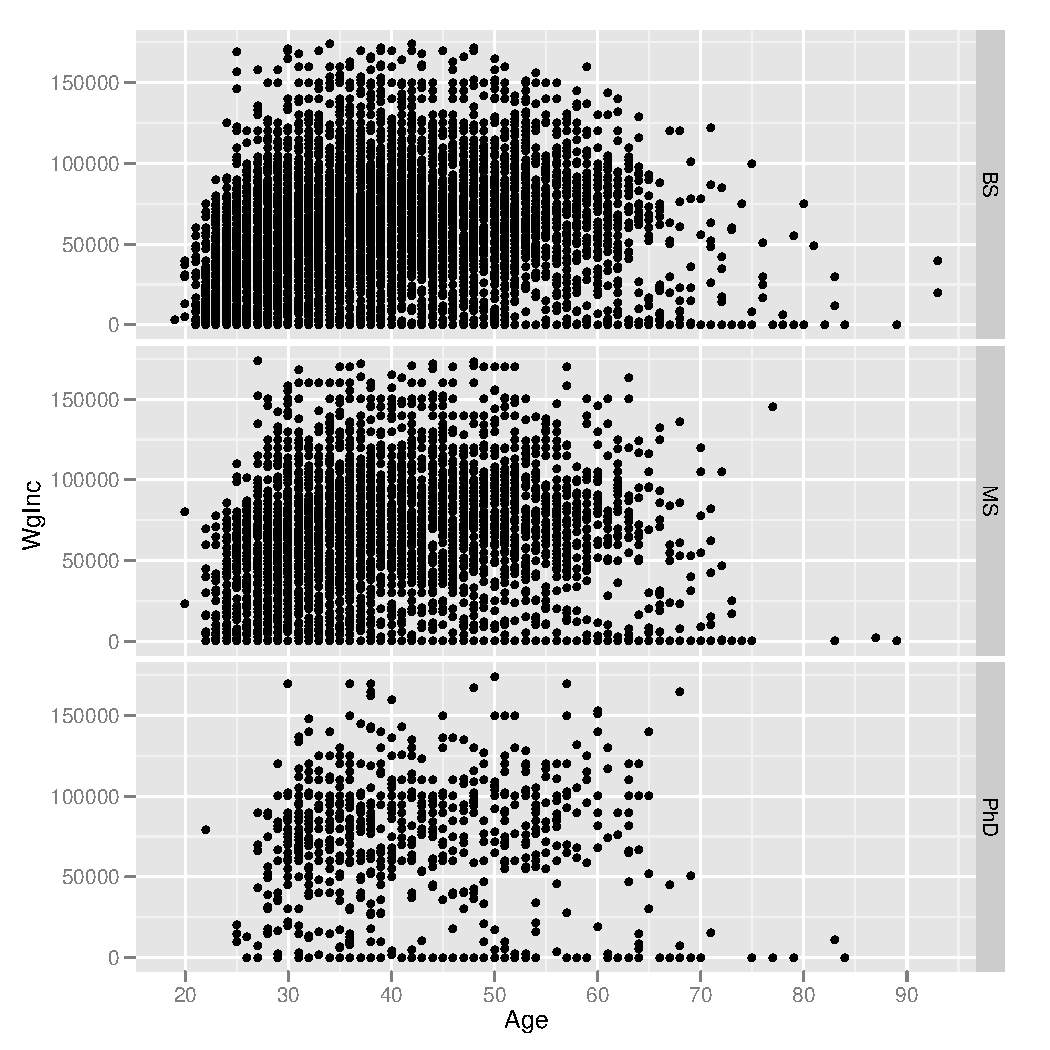
\includegraphics[bb=0 0 504 504,width=4.5in]{FacetVertAgeInc.pdf}

I tried a horizontal presentation too:

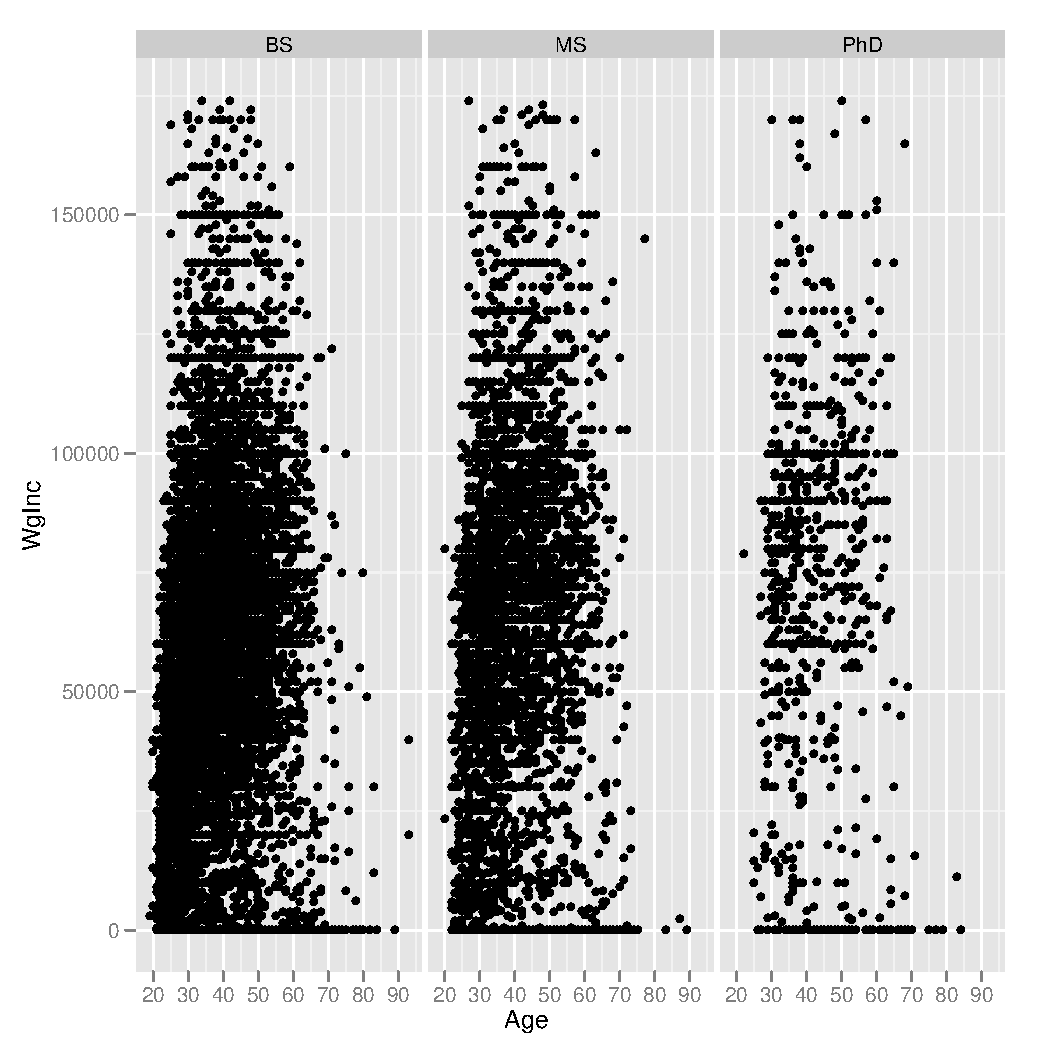
\includegraphics[bb=0 0 504 504,width=4.5in]{FacetHorizAgeInc.pdf}

Note that there doesn't seem to be much relation between degree in
salary, after age 35 or so.

Note that I could have combined operations, e.g.

\begin{lstlisting}
> p + geom_point(aes(x=Age, y=WgInc)) + facet_grid(HiDeg ~ .)
\end{lstlisting}

to get the vertical set of panels, without directly going through the
intermediate step of drawing the nonfaceted graph.

If there had been a Gender variable in the data, I could have defined
rows and columns of panels:

\begin{lstlisting}
> p + geom_point(aes(x=Age, y=WgInc)) + facet_grid(Gender ~ HiDeg)
\end{lstlisting}

\section{Function Plots, Density Estimates and Smoothing}
\label{ggplot2dens}

The {\bf ggplot2} package has lots of ways to plot known functions and
to do smoothing.  Here are some examples:

\begin{lstlisting}
# plot a function
sqfun <- function(t) t^2
# plot over the interval (0,2)
p <- ggplot(data.frame(x=c(0,2)),aes(x))
p + stat_function(fun=sqfun)

# compute and plot a density estimate
w <- rnorm(2500)
p <- ggplot(data.frame(w))
p + geom_density(aes(x=w))  # many other choices
y <- rnorm(2500,sd=2)
p + geom_density(aes(x=w)) + geom_density(aes(x=y))

# generate data from a quadratic function with added noise;
# pretend we don't know it's a quadratic function, and
# smooth the data to get an idea of what the function is like
t <- seq(0.01,2,0.01)
u <- t^2 + rnorm(n=100,sd=0.2)
d <- data.frame(t,u)
p <- ggplot(d)
p + geom_smooth(aes(x=t,y=u),method="loess")
\end{lstlisting}

\section{What's Going on Inside}

In order to use {\bf ggplot2} most effectively, it helps to understand
what happens one level down.  Let's do so via the first example in this
document:

\begin{lstlisting}
> library(ggplot2)
> df1 <- data.frame(u = c(0,2,5), v = c(3:5))
> df1
  u v
1 0 3
2 2 4
3 5 5
> p <- ggplot(df1)
> p
Error: No layers in plot
\end{lstlisting}

By just typing {\bf p}, we meant to print it, but there is nothing to
print for now.  Yet, even at this early stage, {\bf p} has a lot in it:

\begin{lstlisting}
> str(p)
List of 9
 $ data       :'data.frame':	3 obs. of  2 variables:
  ..$ u: num [1:3] 0 2 5
  ..$ v: int [1:3] 3 4 5
 $ layers     : list()
 $ scales     :Reference class 'Scales' [package "ggplot2"] with 1 fields
  ..$ scales: NULL
  ..and 21 methods, of which 9 are possibly relevant:
  ..  add, clone, find, get_scales, has_scale, initialize, input, n,
  ..  non_position_scales
 $ mapping    : list()
 $ theme      : list()
 $ coordinates:List of 1
  ..$ limits:List of 2
  .. ..$ x: NULL
  .. ..$ y: NULL
  ..- attr(*, "class")= chr [1:2] "cartesian" "coord"
 $ facet      :List of 1
  ..$ shrink: logi TRUE
  ..- attr(*, "class")= chr [1:2] "null" "facet"
 $ plot_env   :<environment: R_GlobalEnv> 
 $ labels     : list()
 - attr(*, "class")= chr [1:2] "gg" "ggplot"
\end{lstlisting}

You can see that {\bf p} is indeed a class object, consisting of a list
of various components, some of which themselves are lists.  Note the
{\bf data} component, which sure enough does consist of the data frame
we had specified.

Note by the way that the {\bf layer} component, i.e. {\bf p\$layers}, is
empty, resulting in our failure to plot when we tried to do so above.

Now, let's add a geom:

\begin{lstlisting}
> p1 <- p + geom_line(aes(x=u,y=v))
> str(p1)
List of 9
 $ data       :'data.frame':	3 obs. of  2 variables:
  ..$ u: num [1:3] 0 2 5
  ..$ v: int [1:3] 3 4 5
 $ layers     :List of 1
  ..$ :Classes 'proto', 'environment' <environment: 0x96d8264> 
 $ scales     :Reference class 'Scales' [package "ggplot2"] with 1 fields
  ..$ scales: list()
  ..and 21 methods, of which 9 are possibly relevant:
  ..  add, clone, find, get_scales, has_scale, initialize, input, n,
  ..  non_position_scales
 $ mapping    : list()
 $ theme      : list()
 $ coordinates:List of 1
  ..$ limits:List of 2
  .. ..$ x: NULL
  .. ..$ y: NULL
  ..- attr(*, "class")= chr [1:2] "cartesian" "coord"
 $ facet      :List of 1
  ..$ shrink: logi TRUE
  ..- attr(*, "class")= chr [1:2] "null" "facet"
 $ plot_env   :<environment: R_GlobalEnv> 
 $ labels     :List of 2
  ..$ x: chr "u"
  ..$ y: chr "v"
 - attr(*, "class")= chr [1:2] "gg" "ggplot"
\end{lstlisting}

Now the {\bf layers} component is nonempty, as is the {\bf labels}
component.  

Obviously the rest is complicated, but at least now you have some
understanding of what happens to these class objects when we do ``+''.

Among other things, this insight can help you in debugging, if your {\bf
ggplot2} code doesn't produce what you had expected.

\section{For Further Information}

Just plugging ``ggplot2 tutorial,'' ``ggplot2 introduction,'' ``ggplot2
examples'' and so on into your favorite search engine will give you tons
of information.

Hadley's book, {\it ggplot2: Elegant Graphics for Data Analysis}, is of
course the definitive source, but also try his pictorial reference
manual, at \url{http://had.co.nz/ggplot2/}.  Winston Chang's O'Reilly
series book, the {\it R Graphics Cookbook}, is chock full of examples,
almost all of them using {\bf ggplot2}.  Paul Murrell's book, {\it R
Graphics}, gives a more general treatment of graphics in R.

The {\bf ggobi} packated, whose lead author is UCD professor Duncan
Temple Lang, takes an interactive approach to graphics.

% \end{document}

% pm <- pums[pums$WgInc < 300000,]
% pm$Mas <- pm$Educ == 14
% pm$Bach <- pm$Educ == 13
% pm$PhD <- pm$Educ == 16
% pm$EdCode <- ifelse(pm$Bach,1,ifelse(pm$Mas,2,3))
% pm$HiDeg <- ifelse(pm$EdCode == 1,"BS",ifelse(pm$EdCode == 2,"MS","PhD"))

